\documentclass{article}

\usepackage{titlesec}
\usepackage{longtable}
\usepackage{array} % for defining a new column type
\usepackage{varwidth} %for the varwidth minipage environment
\usepackage{color, colortbl}
\usepackage{caption}
\usepackage{subfigure}
\usepackage{filecontents}
\usepackage[section]{placeins}
\usepackage{float}
\usepackage{lscape}

\definecolor{Gray}{gray}{0.9}

\usepackage{pgf-umlsd}
\usepackage{pgf-umlcd}

\usepackage[latin1]{inputenc}
\usepackage{tikz}
\usetikzlibrary{shapes,arrows}

\newcommand{\sectionbreak}{\clearpage}

\begin{document}


\tikzstyle{decision} = [diamond, draw, fill=blue!20, 
    text width=4.5em, text badly centered, node distance=3cm, inner sep=0pt]
\tikzstyle{block} = [rectangle, draw, fill=blue!20, 
    text width=5em, text centered, rounded corners, minimum height=4em]
\tikzstyle{line} = [draw, -latex']
\tikzstyle{cloud} = [draw, ellipse,fill=red!20, node distance=3cm,
    minimum height=2em]

\newcolumntype{M}{>{\begin{varwidth}{4cm}}l<{\end{varwidth}}} %M is for Maximal column

\begin{titlepage}
	\Huge{Bitcode Assignment 3}
\end{titlepage}


\section{Design Patterns}
Using design patterns in software project is a good practice. It helps to make your software understandable, sustainable and expendable. We have chosen two design patterns and implemented them in our existing code, the state pattern and the strategy pattern.

\subsection{The State Design Pattern}
We chose the state design pattern for the game because the game has become very complex and various objects can and will change a lot of the games behavior and variables.
\paragraph{} With the state design pattern we are able to dictate when certain parts of the game's logic can be executed and when not. This reduces the chances of accidentally changing the games behavior or variables when it is not wanted.
\paragraph{} For example disabling mouse input when the user is in the main menu state makes no sense. Without the state design pattern the disable mouse input (pause game) could be called when it is unwanted. By integrating the pause and resume,into the state design pattern we can choose in which states it is allowed to execute this command. We obviously only want this to happen when the game is running. Otherwhise we throw an exception, allowing easy traceability to where the command was invalidly called, allowing for an easy fix without having to debug the whole program.

\newpage
\subsubsection{State Class Diagram}
The class diagram of the implemented state design mattern is shown in the figure below.
\begin{figure}[H]
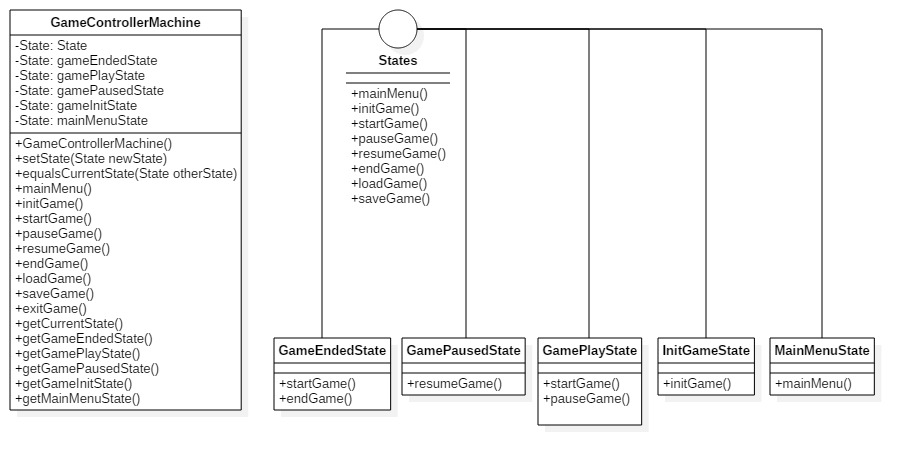
\includegraphics[scale=0.50]{Images/StateMachineClassDiagram.jpg}
\end{figure}

\subsubsection{State Sequence Diagram}
In the figure below the sequence diagram of the implemented state deign pattern is shown.
\begin{figure}[H]
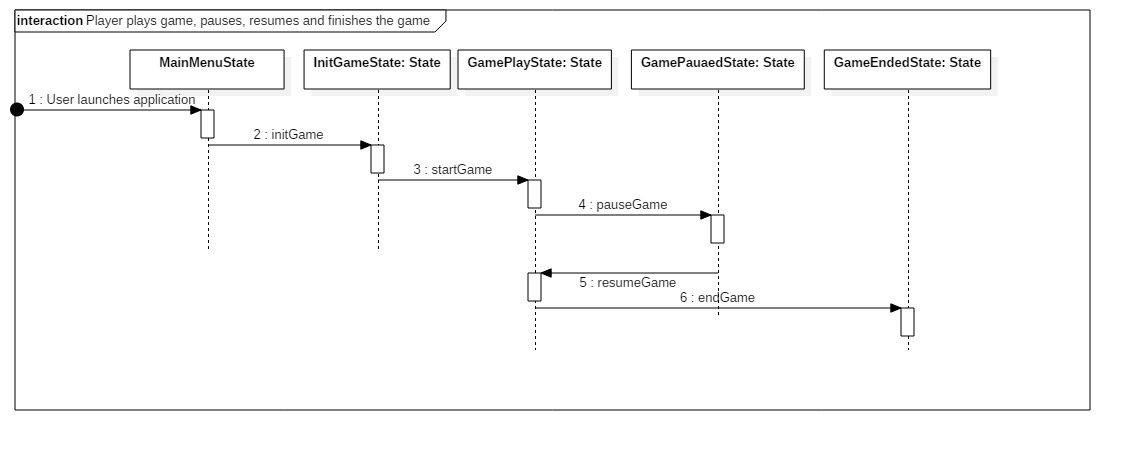
\includegraphics[scale=0.40]{Images/StateMachineSequenceDiagram.jpg}
\end{figure}

\subsection{The Strategy Design Pattern}
The multi-player feature of our game requires handling multiple requests from server. This is the responsibility of the client object to listen to the server and receive these requests and parse them. Based on each request it requires doing an action but there are multiple ways of performing that action and that is why Strategy design pattern comes into play because it helps to encapsulate each request in a separate class and define each class with the same interface so they can be interchangeable.

\subsubsection{Strategy Class Diagram}
There is a general interface called Strategy with one method which accepts two arguments. These arguments will be treated differently based on the implantation. For each request from the server we create a separate class which implements the Strategy interface. And also there is another class called invokeStrategy which is used to map each request to the appropriate implementation. This class has also a method to add a strategy dynamically, so whenever we want to extend our server functionality we don't need to change the base code, we need only to implement a class for handling the request and add it to the invokeStrategy class.


\begin{figure}[H]
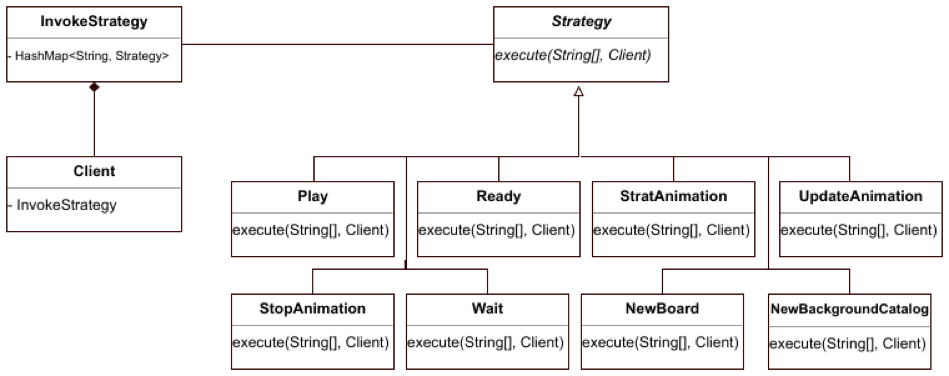
\includegraphics[scale=0.90]{Images/StrategyClassDiagram.png}
\end{figure}

\subsubsection{Strategy Sequence Diagram} 
\begin{figure}[H]
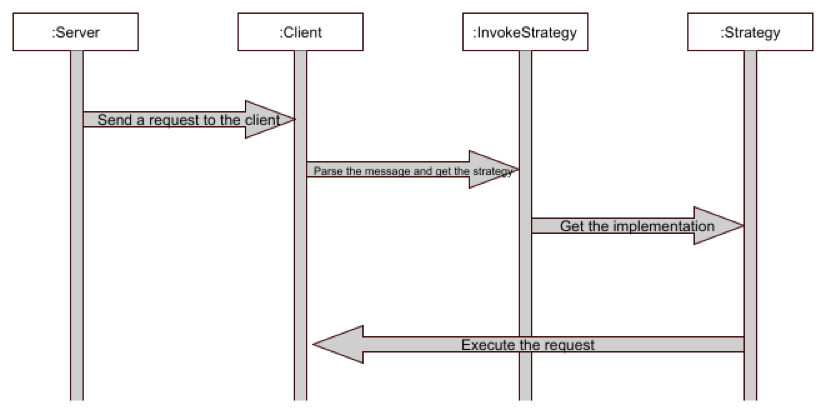
\includegraphics[scale=0.90]{Images/StrategySequenceDiagram.png}
\end{figure}

\newpage
\section{Software Metrics}
keeping track of software metrics helps to keep code clean, understandable, sustainable and expendable. We have chosen to use a intellij plugin called "MetricsReloaded" that helps of measuring software metrics. By running this tool we could compile the following lists of classes and methods that could be improved.

\paragraph{Classes}
\begin{enumerate}
\item StandardItemFactory, WMC: 28
\item MainScreen, DIT: 5
\item Board, WMC: 40
\item Game, WMC: 28
\item BackgroundTileCatalog, WMC: 26
\item ConnectionScreen, DIT: 6
\item JPanelTile, DIT: 5
\item Client, CBO: 23
\item Game, CBO: 21
\item MainScreen, CBO: 20
\end{enumerate}

\paragraph{Methods}
\begin{enumerate}
\item pooralien.Controller.Board.removeGroups, ECC: 6
\item HighScoreTable.HighScoreEnterNameDialog.HighScoreEnterNameDialog, ECC: 4
\item Controller.HighScore.TopXTableModel.getValueAt, ECC: 8
\item pooralien.Controller.BackgroundTileCatalog.BackgroundTileCatalog, ECC: 4
\item pooralien.Controller.BackgroundTile.BackgroundTile, ECC: 4
\item pooralien.Controller.BackgroundTile.equals, ECC: 
\item item.StandardItemFactory.createItem, ECC: 8
\item item.StandardItemFactory.createRandomItem, ECC: 8
\end{enumerate}

\paragraph{} For each improvable class or method a issue is created on our github repository so that everyone can help improve the code. 

\newpage
\section{Defensive Programming}
In the previous assignments it was required to use a game configuration file for initializing variables using a provided library. However, the provided library introduced bugs in the game. 
\paragraph{} To solve the bugs we have created a wrapper class (CameConfig) around the library's API that catches all the bugs and checks if the variables are within limits. This means that for every different API call we created a method in the GameConfig class. In the sequence diagram below is shown how the wrapper class works.

\begin{figure}[H]
	\centering
	\begin{sequencediagram}
		\newthread{A}{:Launcher}{}
		\newthread{B}{:GameConfig}{}
		\newthread{C}{:DefProAPI}{}
		\begin{call}{A}{getString()}{B}{}
			\begin{call}{B}{getStringValue()}{C}{}
			\end{call}
		\end{call}
	\end{sequencediagram}
\end{figure}

\paragraph{} In every method in the CameConfig class that implements the API checks are build in to verify the data that is returned by the API. Also if the API throws an exception it is catched in the method. If an exception occurs or the data returned by the API is not within the defined boundaries the method will return the defined default value. The flowchart below shows how the method getString() is implemented.

\begin{tikzpicture}[node distance = 2cm, auto]
    % Place nodes
    \node [block] (defpro) {getString ValueOf()};
    \node [cloud, left of=defpro] (start) {getString()};
	\node [decision, below of=defpro] (exception) {no exception?};
	\node [decision, below of=exception] (limit) {within limits?};
	\node [decision, below of=limit] (alpha) {is alphabetic?};
	\node [block, left of=alpha, node distance=3cm] (default) {return default value};
    \node [block, right of=alpha, node distance=3cm] (config) {return config value};
    
    \path [line,dashed] (start) -- (defpro);
    \path [line] (defpro) -- (exception);
	\path [line] (exception) -- node {yes}(limit);
	\path [line] (limit) -- node {yes}(alpha);
	\path [line] (alpha) -- node {no}(default);
	\path [line] (alpha) -- node {yes}(config);
	
	\path [line] (exception) -| node {no}(default);
	\path [line] (limit) -| node {no}(default);
    
\end{tikzpicture}  

\paragraph{} In this particular example the following conditions makes the method return the defined default value.
\begin{itemize}
	\item If the library thorows an exception.
	\item If the amount of characters in the sting is less or more then expected.
	\item If the string is not alphabetic.
\end{itemize}

\section{Selectable Difficulty}
One way of making the game more competitive is to implement selectable difficulty. The idea is that the user can select a desired difficultly between easy, normal and hard before the game starts. The selected level of difficulty will noticeably influence the difficulty of the game.   

\subsection{Requirements}
The requirements are ordered by the MoSCoW model.

\paragraph{Must Have:}
\begin{itemize}
	\item The game must have three levels of difficulty, easy, normal and hard.
	\item The player must be able to select the desired difficulty befor the game starts.
	\item The game must have a start screen.
\end{itemize}

\paragraph{Should Have:}
\begin{itemize}
	\item The player should get more points when removing a tile or a background tile when the game is more difficult.
\end{itemize}


\paragraph{Could Have:}
\begin{itemize}
	\item Higher difficulty could mean that the player should find four of the same tiles on a row.
	\item Higher difficulty could mean that the player has less moves to remove all background tiles.
	\item Higher difficulty could mean that there are more background tiles. 
	\item Lower difficulty could mean six different tiles instead of 7 tiles.
\end{itemize}


\newpage
\subsection{Software Design}
The figure below shows the class diagram of the implementation.
\begin{figure}[H]
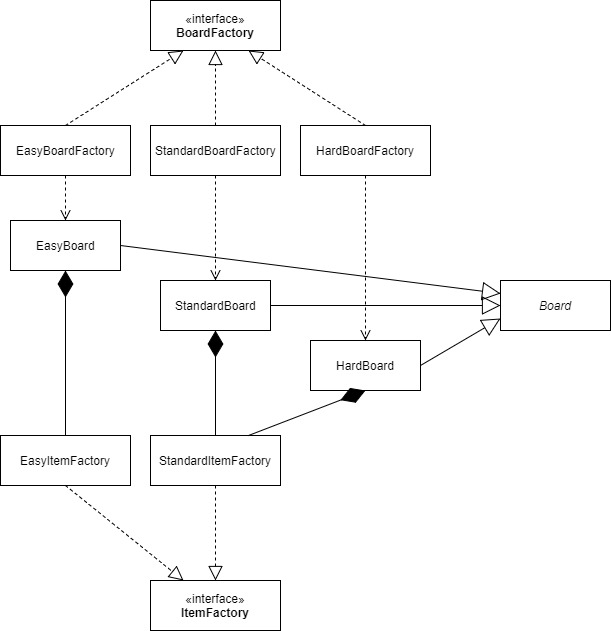
\includegraphics[scale=0.55]{Images/DifficultiesClassDiagram.jpg}
\end{figure}


\end{document}



